\chapter{Przebiegi odpowiedzi skokowych użytecznych w algorytmie DMC}
Aby otrzymać odpowiedź skokową wykorzystywaną w algorytmie DMC, należy postępować analogicznie - należy pobudzić obiekt skokiem jednostkowym, gdzie od chwili zerowej sygnał sterujący ma wartość 1, a w przeszłości jest zerowy. Wynik tej odpowiedzi skokowej jest przedstawiony na Rys.~\ref{skokDMC}.
\begin{figure}
	\centering
	\caption{ }
	% This file was created by matlab2tikz.
%
\definecolor{mycolor1}{rgb}{0.00000,0.44700,0.74100}%
\definecolor{mycolor2}{rgb}{0.85000,0.32500,0.09800}%
%
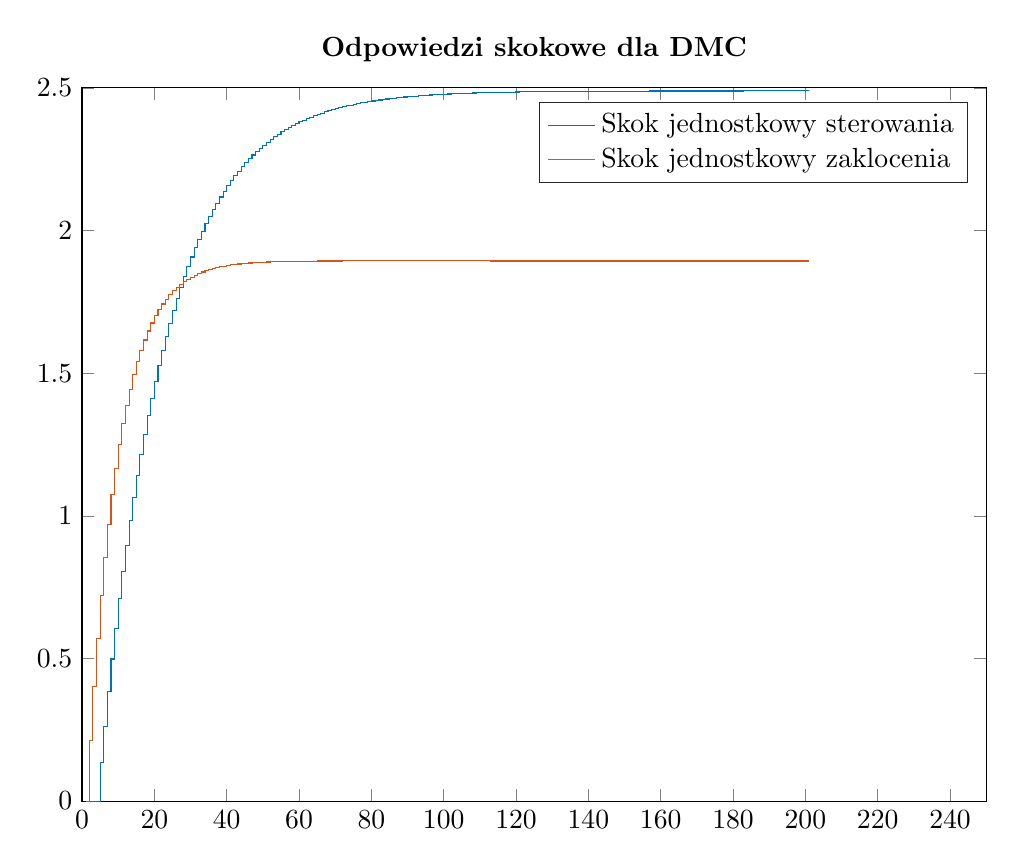
\begin{tikzpicture}

\begin{axis}[%
width=4.521in,
height=3.566in,
at={(0.758in,0.481in)},
scale only axis,
xmin=0,
xmax=250,
ymin=0,
ymax=2.5,
axis background/.style={fill=white},
title style={font=\bfseries},
title={Odpowiedzi skokowe dla DMC},
legend style={legend cell align=left, align=left, draw=white!15!black}
]
\addplot[const plot, color=mycolor1] table[row sep=crcr] {%
1	0\\
2	0\\
3	0\\
4	0\\
5	0.1351\\
6	0.26289287\\
7	0.383771026719\\
8	0.49810612839733\\
9	0.606250137113836\\
10	0.708536330858846\\
11	0.805280267249039\\
12	0.896780700762612\\
13	0.983320455355331\\
14	1.06516725429164\\
15	1.14257450899172\\
16	1.21578206865655\\
17	1.28501693238935\\
18	1.35049392548527\\
19	1.41241634151109\\
20	1.47097655174561\\
21	1.52635658349832\\
22	1.57872866877043\\
23	1.62825576466828\\
24	1.67509204692551\\
25	1.71938337783653\\
26	1.76126774985127\\
27	1.80087570602894\\
28	1.83833073849766\\
29	1.87374966601712\\
30	1.90724299169265\\
31	1.93891524184229\\
32	1.96886528697263\\
33	1.99718664577498\\
34	2.02396777301084\\
35	2.0492923321146\\
36	2.07323945330177\\
37	2.09588397793294\\
38	2.11729668984733\\
39	2.13754453434475\\
40	2.15669082546108\\
41	2.17479544215061\\
42	2.19191501395761\\
43	2.2081030967304\\
44	2.22341033890308\\
45	2.23788463884336\\
46	2.25157129373964\\
47	2.26451314047612\\
48	2.27675068892145\\
49	2.28832224803482\\
50	2.2992640451721\\
51	2.30961033895493\\
52	2.31939352604657\\
53	2.32864424216063\\
54	2.33739145761131\\
55	2.34566256769777\\
56	2.35348347820001\\
57	2.36087868624844\\
58	2.36787135681618\\
59	2.37448339506926\\
60	2.38073551479783\\
61	2.38664730313958\\
62	2.39223728179497\\
63	2.39752296492385\\
64	2.40252091390226\\
65	2.40724678910918\\
66	2.41171539890352\\
67	2.41594074594339\\
68	2.41993607099121\\
69	2.42371389434078\\
70	2.42728605499498\\
71	2.43066374771585\\
72	2.43385755806232\\
73	2.43687749552458\\
74	2.43973302485827\\
75	2.44243309571602\\
76	2.44498617066874\\
77	2.44740025170392\\
78	2.44968290528357\\
79	2.45184128604005\\
80	2.45388215918354\\
81	2.4558119216913\\
82	2.45763662234458\\
83	2.45936198067612\\
84	2.46099340488705\\
85	2.46253600878939\\
86	2.463994627827\\
87	2.46537383422513\\
88	2.46667795131579\\
89	2.46791106708384\\
90	2.46907704697614\\
91	2.47017954601382\\
92	2.47122202024545\\
93	2.47220773757713\\
94	2.47313978801326\\
95	2.47402109334002\\
96	2.47485441628193\\
97	2.47564236916017\\
98	2.4763874220796\\
99	2.47709191067034\\
100	2.47775804340797\\
101	2.47838790853536\\
102	2.47898348060771\\
103	2.47954662668144\\
104	2.48007911216621\\
105	2.48058260635838\\
106	2.48105868767329\\
107	2.48150884859281\\
108	2.48193450034349\\
109	2.4823369773201\\
110	2.4827175412684\\
111	2.48307738524023\\
112	2.48341763733321\\
113	2.48373936422702\\
114	2.48404357452703\\
115	2.484331221926\\
116	2.48460320819366\\
117	2.48486038600347\\
118	2.48510356160561\\
119	2.48533349735436\\
120	2.48555091409791\\
121	2.48575649343812\\
122	2.4859508798672\\
123	2.48613468278808\\
124	2.48630847842483\\
125	2.48647281162901\\
126	2.48662819758773\\
127	2.48677512343869\\
128	2.48691404979732\\
129	2.48704541220078\\
130	2.48716962247327\\
131	2.48728707001715\\
132	2.48739812303362\\
133	2.48750312967704\\
134	2.48760241914639\\
135	2.48769630271725\\
136	2.48778507471768\\
137	2.48786901345089\\
138	2.48794838206773\\
139	2.48802342939168\\
140	2.48809439069886\\
141	2.48816148845566\\
142	2.48822493301615\\
143	2.48828492328154\\
144	2.48834164732372\\
145	2.4883952829749\\
146	2.4884459983851\\
147	2.48849395254926\\
148	2.48853929580575\\
149	2.48858217030766\\
150	2.48862271046845\\
151	2.48866104338333\\
152	2.48869728922771\\
153	2.48873156163396\\
154	2.48876396804766\\
155	2.48879461006441\\
156	2.48882358374836\\
157	2.48885097993338\\
158	2.48887688450781\\
159	2.48890137868371\\
160	2.48892453925151\\
161	2.4889464388207\\
162	2.48896714604749\\
163	2.48898672585005\\
164	2.48900523961201\\
165	2.48902274537493\\
166	2.48903929802024\\
167	2.48905494944131\\
168	2.4890697487061\\
169	2.48908374221106\\
170	2.48909697382653\\
171	2.48910948503428\\
172	2.48912131505758\\
173	2.48913250098415\\
174	2.48914307788243\\
175	2.48915307891153\\
176	2.48916253542518\\
177	2.48917147707005\\
178	2.48917993187863\\
179	2.48918792635719\\
180	2.48919548556882\\
181	2.48920263321205\\
182	2.48920939169509\\
183	2.48921578220614\\
184	2.48922182477978\\
185	2.48922753835979\\
186	2.48923294085854\\
187	2.48923804921313\\
188	2.48924287943852\\
189	2.48924744667773\\
190	2.48925176524927\\
191	2.4892558486921\\
192	2.48925970980802\\
193	2.48926336070183\\
194	2.48926681281926\\
195	2.48927007698289\\
196	2.48927316342604\\
197	2.48927608182487\\
198	2.48927884132871\\
199	2.48928145058875\\
200	2.48928391778515\\
201	2.4892862506527\\
};
\addlegendentry{Skok jednostkowy sterowania}

\addplot[const plot, color=mycolor2] table[row sep=crcr] {%
1	0\\
2	0.21325\\
3	0.402566525\\
4	0.5706310193925\\
5	0.719824758230277\\
6	0.852262435391232\\
7	0.969821994062698\\
8	1.07417111989557\\
9	1.16679077015859\\
10	1.2489960704627\\
11	1.32195487353598\\
12	1.38670424158905\\
13	1.44416508455507\\
14	1.49515516050455\\
15	1.5404006214587\\
16	1.5805462673287\\
17	1.61616465250584\\
18	1.64776417345998\\
19	1.6757962513457\\
20	1.70066171086264\\
21	1.72271644529123\\
22	1.74227644756518\\
23	1.75962227830916\\
24	1.77500303383474\\
25	1.78863987004151\\
26	1.80072913191104\\
27	1.81144513272312\\
28	1.82094262218681\\
29	1.8293589782944\\
30	1.83681615381219\\
31	1.84342240486355\\
32	1.84927382598836\\
33	1.85445571333449\\
34	1.85904377521469\\
35	1.86310520711001\\
36	1.86669964629008\\
37	1.8698800195232\\
38	1.87269329584175\\
39	1.87518115498963\\
40	1.87738058098954\\
41	1.87932438921178\\
42	1.88104169438843\\
43	1.88255832618391\\
44	1.88389719819297\\
45	1.88507863558047\\
46	1.88612066599343\\
47	1.88703927785803\\
48	1.88784864971365\\
49	1.88856135382752\\
50	1.8891885369705\\
51	1.889740080912\\
52	1.89022474490587\\
53	1.89065029218481\\
54	1.89102360225478\\
55	1.89135077058071\\
56	1.89163719707631\\
57	1.89188766465286\\
58	1.89210640894123\\
59	1.8922971801767\\
60	1.89246329812527\\
61	1.89260770083171\\
62	1.89273298788249\\
63	1.89284145879866\\
64	1.89293514710527\\
65	1.8930158505624\\
66	1.89308515798875\\
67	1.89314447306016\\
68	1.89319503542305\\
69	1.89323793942406\\
70	1.89327415072397\\
71	1.89330452103361\\
72	1.89332980118285\\
73	1.89335065271018\\
74	1.89336765813931\\
75	1.89338133009057\\
76	1.89339211935827\\
77	1.8934004220705\\
78	1.89340658603479\\
79	1.89341091636141\\
80	1.89341368044576\\
81	1.89341511238225\\
82	1.89341541687378\\
83	1.89341477269396\\
84	1.89341333575249\\
85	1.89341124180867\\
86	1.89340860887298\\
87	1.89340553933188\\
88	1.89340212182743\\
89	1.89339843291944\\
90	1.89339453855492\\
91	1.89339049536674\\
92	1.89338635182096\\
93	1.89338214923005\\
94	1.89337792264742\\
95	1.89337370165668\\
96	1.89336951106777\\
97	1.89336537153071\\
98	1.89336130007626\\
99	1.89335731059206\\
100	1.89335341424162\\
101	1.89334961983275\\
102	1.89334593414135\\
103	1.89334236219565\\
104	1.89333890752559\\
105	1.8933355723814\\
106	1.89333235792485\\
107	1.89332926439662\\
108	1.89332629126238\\
109	1.89332343734019\\
110	1.89332070091147\\
111	1.89331807981744\\
112	1.8933155715428\\
113	1.89331317328814\\
114	1.89331088203254\\
115	1.89330869458742\\
116	1.89330660764285\\
117	1.89330461780712\\
118	1.89330272164053\\
119	1.893300915684\\
120	1.89329919648324\\
121	1.89329756060906\\
122	1.89329600467417\\
123	1.89329452534715\\
124	1.89329311936374\\
125	1.89329178353601\\
126	1.8932905147595\\
127	1.8932893100188\\
128	1.89328816639159\\
129	1.89328708105157\\
130	1.89328605127027\\
131	1.89328507441799\\
132	1.89328414796402\\
133	1.89328326947613\\
134	1.89328243661968\\
135	1.89328164715615\\
136	1.89328089894139\\
137	1.89328018992356\\
138	1.89327951814085\\
139	1.89327888171896\\
140	1.89327827886856\\
141	1.89327770788251\\
142	1.89327716713313\\
143	1.89327665506937\\
144	1.89327617021397\\
145	1.89327571116066\\
146	1.8932752765713\\
147	1.89327486517319\\
148	1.89327447575627\\
149	1.89327410717047\\
150	1.89327375832314\\
151	1.89327342817645\\
152	1.89327311574496\\
153	1.89327282009324\\
154	1.89327254033352\\
155	1.89327227562346\\
156	1.89327202516406\\
157	1.89327178819751\\
158	1.89327156400525\\
159	1.89327135190604\\
160	1.89327115125414\\
161	1.89327096143754\\
162	1.8932707818763\\
163	1.89327061202094\\
164	1.89327045135091\\
165	1.89327029937309\\
166	1.89327015562046\\
167	1.8932700196507\\
168	1.89326989104499\\
169	1.89326976940674\\
170	1.89326965436046\\
171	1.8932695455507\\
172	1.89326944264094\\
173	1.89326934531267\\
174	1.89326925326441\\
175	1.89326916621082\\
176	1.89326908388186\\
177	1.89326900602199\\
178	1.89326893238937\\
179	1.89326886275518\\
180	1.89326879690291\\
181	1.89326873462769\\
182	1.8932686757357\\
183	1.89326862004356\\
184	1.8932685673778\\
185	1.89326851757429\\
186	1.89326847047777\\
187	1.89326842594138\\
188	1.89326838382618\\
189	1.89326834400075\\
190	1.89326830634079\\
191	1.89326827072872\\
192	1.89326823705332\\
193	1.8932682052094\\
194	1.89326817509747\\
195	1.89326814662343\\
196	1.89326811969828\\
197	1.89326809423785\\
198	1.89326807016252\\
199	1.89326804739701\\
200	1.89326802587012\\
201	1.8932680055145\\
};
\addlegendentry{Skok jednostkowy zaklocenia}

\end{axis}
\end{tikzpicture}%
	\label{skokDMC}
\end{figure}